% Use UTF-8 encoding!!
% (c) Stefan Ulbrich, 2012
% updated in May, 2015 by Michael Bechtel

\documentclass[english,ngerman]{KITreprt}

%% --------------------------------
%% Obligatory Parameters:
%% --------------------------------

\renewcommand{\mythesis}{\bachelorsthesis} %\mastersthesis, \bachelorsthesis, \protocol, \studienarbeit, \diplomarbeit
\renewcommand{\mytitle}{ \iflanguage{english}{Robust Regrasping-Actions on Humanoid Robots}{Robust Regrasping-Actions on Humanoid Robots} }
\renewcommand{\myname}{Stefan Reither}
%\renewcommand{\myshorttitle}{Die offizielle \LaTeX-Vorlage des HIS}
\renewcommand{\myshorttitle}{}
\cfoot{\mytitle}

\renewcommand{\timestart}{4. November 2011}
\renewcommand{\timeend}{\iflanguage{english}{February 7\textsuperscript{th},}{7. Februar} 2010}
\newcommand{\referee}{Erstgutachter}
\newcommand{\refereetwo}{Zweitgutachter}
%\newcommand{\refereethree}{Drittgutachter}

\newcommand{\advisor}{Dr.-Ing. Mirko Wächter}
\newcommand{\advisortwo}{Dr.-Ing. Nikolaus Vahrenkamp}
%\newcommand{\advisorthree}{Betreuender Mitarbeiter 3}

\graphicspath{{./images/}}


%% -------------------------------
%% |  Information for PDF file   |
%% -------------------------------
\hypersetup{
	pdfauthor={\myname},
	pdftitle={\mytitle},
	pdfsubject={Not set},
	pdfkeywords={Not set}
}




\begin{document}


\selectlanguage{ngerman}
%\selectlanguage{english}


\maketitle

\thispagestyle{empty}
\newpage
%\topskip0pt
\vspace*{\fill}
\noindent
\textbf{Erkl\"arung:}\\
\\
\noindent
Ich versichere hiermit, dass ich die Arbeit selbstst\"andig verfasst habe, keine anderen als die angegebenen Quellen und Hilfsmittel benutzt habe, die w\"ortlich oder inhaltlich \"ubernommenen
Stellen als solche kenntlich gemacht habe und die Satzung des Karlsruher Instituts f\"ur Technologie zur Sicherung guter wissenschaftlicher Praxis beachtet habe.\\
\\
\\
\noindent
Karlsruhe, den \timeend 
\begin{flushright}

\myname
\end{flushright}

\vspace*{\fill}
\cleardoublepage



\thispagestyle{empty}
\newpage
%\topskip0pt
\vspace*{\fill}
\noindent
\textbf{Abstract:}\\
\\
\noindent
English abstract goes here.
\vspace*{\fill}
\cleardoublepage


\thispagestyle{empty}
\newpage
%\topskip0pt
\vspace*{\fill}
\noindent
\textbf{Kurzzusammenfassung:}\\
\\
\noindent
Deutsche Kurzzusammenfassung hier.
\vspace*{\fill}
\cleardoublepage


\tableofcontents
\setcounter{page}{1}


\chapter{Einleitung}
\section{Einleitungtest}

\textbf{Hello world!}
 
Hello, here is some text without a meaning.  This... 

\documentclass[../main.tex]{subfiles}

\begin{document}
StandDerTechnik
\end{document}
\chapter{Grundlagen}

In diesem Kapitel sollen einige grundlegenden Themen angesprochen werden, die dann im darauffolgenden Kapitel als bekannt vorausgesetzt werden. Dazu gehören zu einen Algorithmen, die in dieser Arbeit verwendet werden, aber nicht im Rahmen dieser entwickelt wurden. Zum anderen wird ein Überblick über das Framework gegeben, in das das entwickelte System eingebettet ist. Außerdem wird der Roboter an dem die Evaluation vorgenommen werden wird vorgestellt.

\section{Das ArmarX-Framework}
\subsection{Allgemeine Struktur und Funktionalitäten}

Das ArmarX-Framework ist ein sogenanntes \glqq Robot Development Environment\grqq{} (RDE). Ein Programm mit dem ohne viel Training des Benutzers und auf einem hohen Abstraktionsniveau Ansteuerungsprogramme für, in diesem Fall, humanoide Roboter erstellt werden können. Dieses Framework (\textcolor{red}{Referenz}) wird am Karlsruher Institut für Technologie (KIT) seit dem Jahr 2011 entwickelt und ist noch immer in der Weiterentwicklung. \\
Eine der Hauptaufgaben von RDEs ist dabei die Kommunikation zum einen zwischen der Hardware und der Software und zum anderen zwischen einzelnen Komponenten der Robotersteuerung. Hier wird dafür die Middleware \glqq Ice\grqq{} \textcolor{red}{Korrekter Name + Referenz} verwendet, die über das lokale Netzwerk erlaubt Komponenten auf verschiedenen Maschinen laufen zu lassen, die aber dennoch miteinander kommunizieren können. Das erlaubt eine bequeme Steuerung des Roboters von außerhalb: Die Lowlevel-Controller und die Hardware-Abstraktionen können auf den im Roboter verbauten PCs arbeiten, während auf einem externen PC rechenintensive Operationen wie Kinematik, Bildverarbeitung und die Highlevel-Robotersteuerung ausgeführt werden.
\\

ArmarX ist in drei Schichten unterteilt (vgl. Abb. \ref{fig:ArmarX_structure}): Zum Einen die bereits erwähnte Middleware-Schicht, die Funktionalitäten zur einfachen Erstellung von verteilten Anwendungen bietet. Außerdem das sogenannte \glqq Robot Framework Layer\grqq{}, welches grundlegende Funktionalitäten für die Robotersteuerung bereitstellt und schließlich die Anwendung-Schicht in der komplexe Roboterprogramme erstellt werden können.

\begin{figure}[h]
\begin{center}
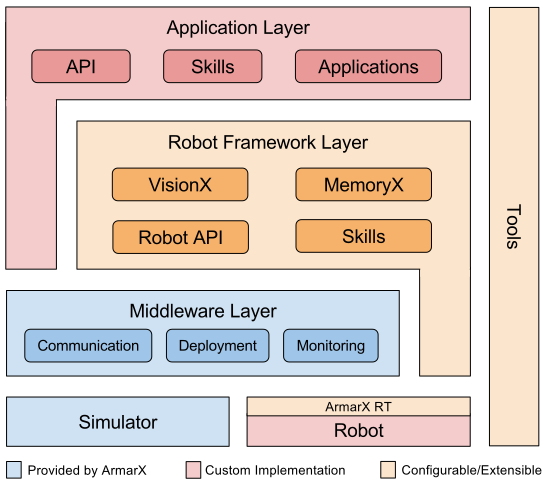
\includegraphics[width=0.7\textwidth]{ArmarX_Structure}
\caption{Fehlt}
\label{fig:ArmarX_structure}
\end{center}
\end{figure}

\paragraph{Middleware-Schicht} Jeder Programmbaustein in ArmarX ist eine Komponente, die einen geregelten Lebenszyklus hat. Zunächst wird die Komponente erstellt und dann auf mögliche Abhängigkeiten gewartet. Diese Abhängigkeiten sind in der Regel andere Komponenten die erst vollständig gestartet sein müssen, bevor die aktuelle Komponente selbst in den \textit{Connected}-Zustand übergehen kann. Falls eine Komponente im Laufe des Betriebs ausfällt, erkennt die Middleware-Schicht dies und bringt jede Komponente, die eine Abhängigkeit auf das fehlerhafte Objekt hat, in einen Wartezustand. Damit ist garantiert, dass zu keinem Zeitpunkt ein Methodenaufruf auf einem nicht korrekt laufenden Objekt getätigt wird. Somit wird verhindert, dass eine einzelne Komponente das gesamte Programm zum Absturz bringen kann. \\
Die Middleware-Schicht bietet darüber hinaus ein Interface zu Entwicklung von ArmarX-Komponenten. Diese können in drei Kategorien unterteilt werden: Die \glqq Sensor-Actor Units\grqq{}, die zur Abstraktion und Ansteuerung von Endgeräten wie zum Beispiel Kameras oder Robotergelenken dienen. Die \glqq Observers\grqq{}, die Sensor-Werte auswerten und basierend auf der Erfüllbarkeit von Bedingungen (z.B. dass die Motortemperatur eines Gelenks einen kritischen Wert überschreitet) Ereignisse an andere Komponenten schicken können. Und schließlich die \glqq Statecharts\grqq{}~(\ref{sec:Statechart_concept}), die komplexe Roboter-Programme darstellen.

\paragraph{\glqq Robot Framework\grqq -Schicht} In dieser Schicht finden sich alle konfigurierbaren Komponenten die die Interaktion mit dem Roboter realisieren. Das interne Model des Roboters mit dessen physikalischen Attributen, seinen Sensoren und seiner kinematischen Struktur ist aus dem gesamten Netzwerk erreichbar und erlaubt somit spezialisierte Komponenten für beispielsweise Griffplanung, Bewegungsplanung, Koordinatentransformationen zwischen verschiedenen Koordinatensystemen des Roboters, Berechnung der Vorwärts- und Rückwärtskinematik~(\autoref{sec:InverseKinematik}) oder Kollisionserkennung. \\
Für viele dieser Anforderungen ist es unerlässlich, dass der Roboter Wissen über den Zustand der Umwelt hat. In \textit{MemoryX} werden in einer nicht-relationalen Datenbank Informationen über bekannte Objekte und deren Beziehungen untereinander gespeichert. Dieser Speicherabschnitt wird \textit{Prior Knowledge} genannt. Das Wissen darin ist statisch und dem Roboter zu jedem Zeitpunkt bekannt. Basierend darauf und optischen Sensordaten kann nun eine vermutete Modellierung der Umwelt im sog. \textit{Working Memory} generiert werden. Der Zustand in diesem Speichersegment wird durch Objektlokalisierung und Selbstlokalisierung des Roboters fortlaufend aktualisiert. \\



\subsection{\textcolor{red}{Das Statechart-Konzept}}\label{sec:Statechart_concept}

\section{Der Humanoide Roboter ARMAR-IIIa}

\section{Inverse Kinematik}\label{sec:InverseKinematik}
\subsection{Constrained IK}\label{sec:ConstrainedIK}

\section{Bewegungsplanung} \label{sec:Bewegungsplanung}
\subsection{Rapidly-exploring random tree}

\section{Visual-Servoing}
\subsection{Objekterkennung}
\subsection{Objektverfolgung}
\chapter{\textcolor{red}{Methodik (besserer Name benötigt)}}

\section{Gesamtstruktur}

\section{Griffauswahl}

\section{Objektverfolgung und Objektpose-Bestimmung}

\section{Statechart}
\chapter{Evaluation und Testergebnisse}
\chapter{Zusammenfassung und Ausblick}


\bibliographystyle{dinat} %-Deutsch

\bibliography{LiteraturVerzeichnis}

\end{document}
